\section{Evaluation}
\label{sec:evaluation}

In this section, we evaluate the effectiveness of our proposed technique by showing that different ML models (e.g., SVM, NNs, GP) have much higher loss (or error rates)  in the  identified ``unconfident'' regions.  However, one thing we should point out is  that, for classification problems,  ``unconfident'' regions do not always mean lower error rates. For example, Figure~\ref{fig:toy3} shows a binary classification problem where the decision boundary is a circle.  The SVM classifier has very high accuracy in the feature space far from the circle decision boundaries, even though it has learned very few or no training samples from these regions.  
\begin{figure}[t]
\centering
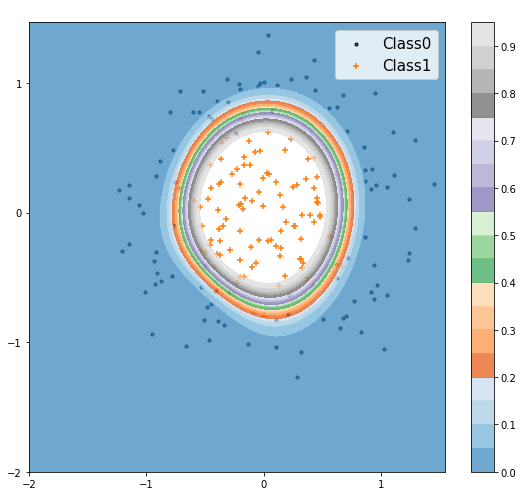
\includegraphics[width=0.4\textwidth]{FIG/toy3.png}
\caption{A binary classification toy  example}
\label{fig:toy3}
\end{figure}


\subsection{Classification Problems}

\subsubsection{The Navigation Task for Mobile Robot SCITOS-G5~\cite{Dua:2017}}




\subsection{Regression Problems}

\subsubsection{The Inverse Dynamics of a  SARCOS Robot Arm~\cite{SARCOS}}
The task is to map from a 21-dimensional input space (7 joint positions, 7 joint velocities, 7 joint accelerations) to the corresponding torque.


\begin{figure}[h]
\centering
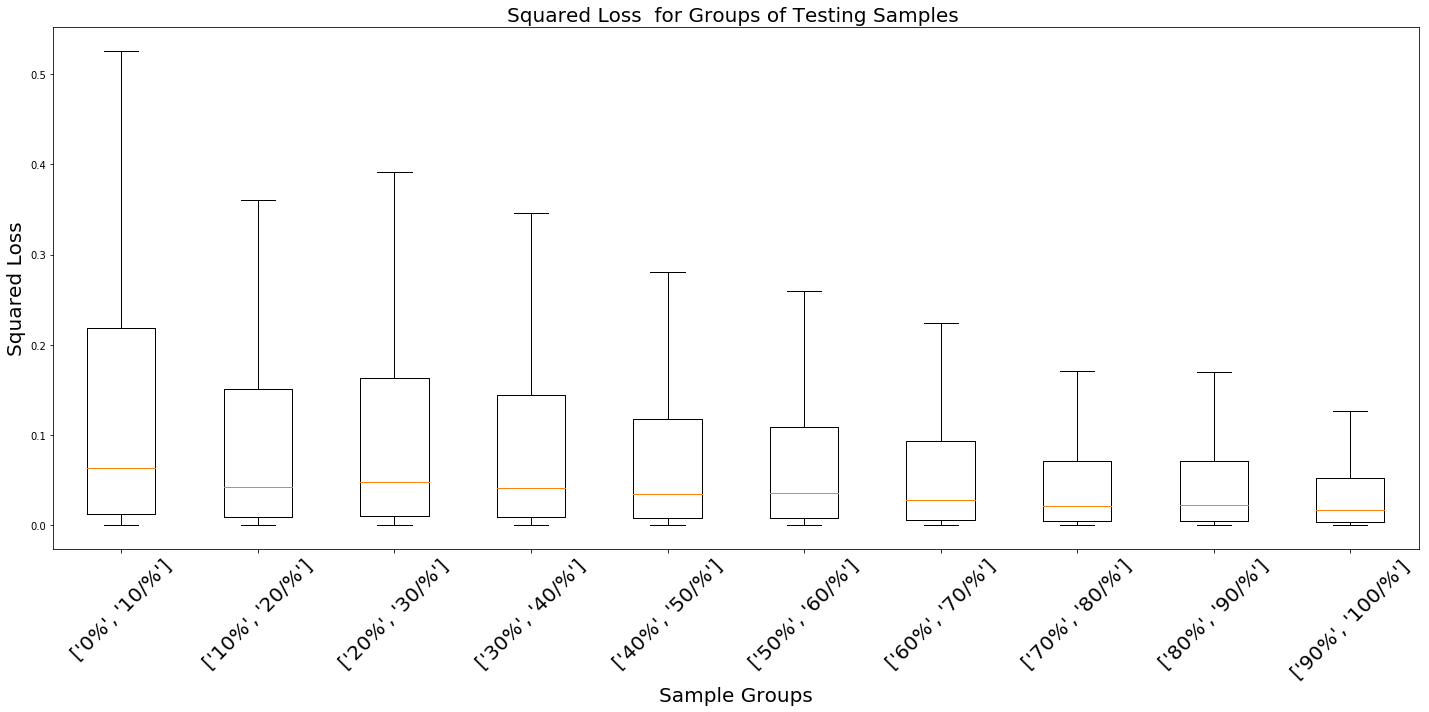
\includegraphics[width=0.5\textwidth]{PLT/sarcos_mlpbox.png}
\caption{SARCO: box plot of mean squared loss of NNs}
\label{fig:sarcos_mlpbox}
\end{figure}

\begin{figure}[h]
\centering
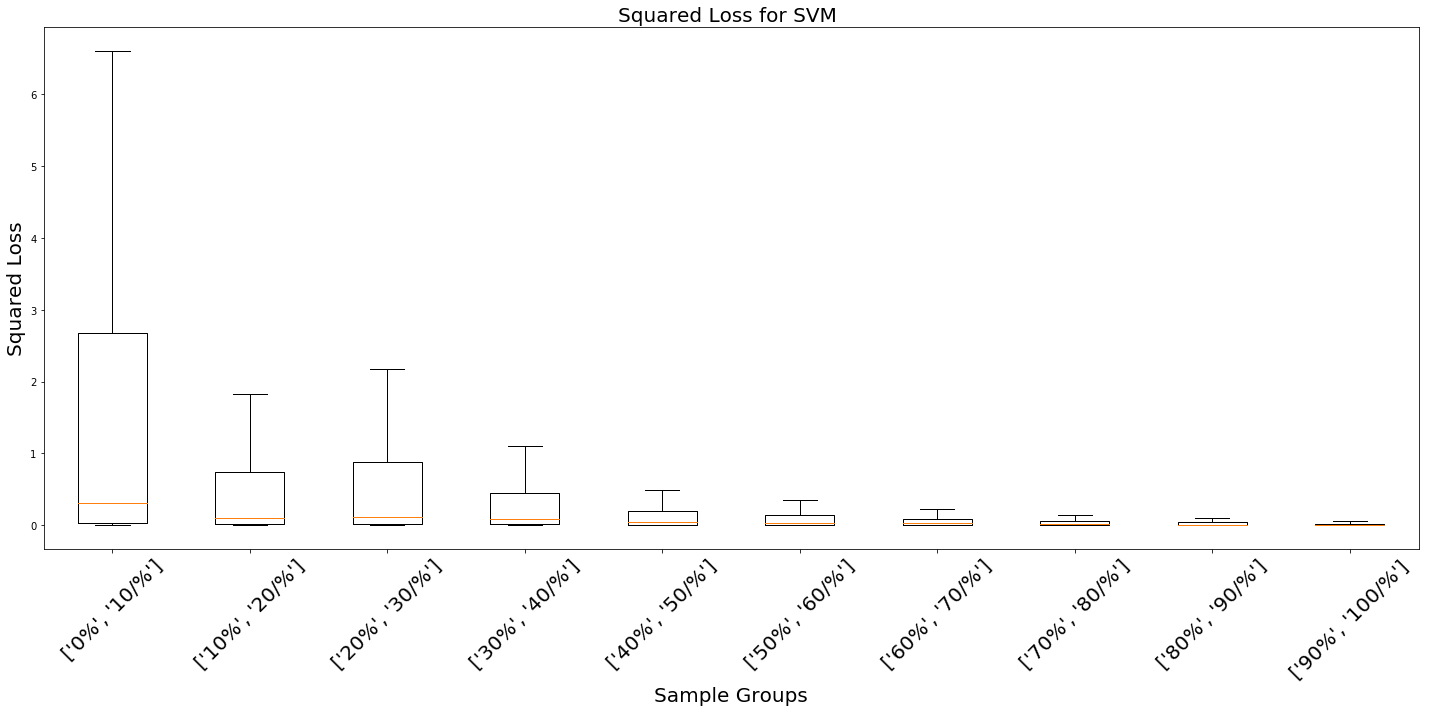
\includegraphics[width=0.5\textwidth]{PLT/sarcos_svmbox.png}
\caption{SARCO: box plot of mean squared loss of SVM}
\label{fig:sarcos_svmbox}
\end{figure}


\begin{figure}[h]
\centering
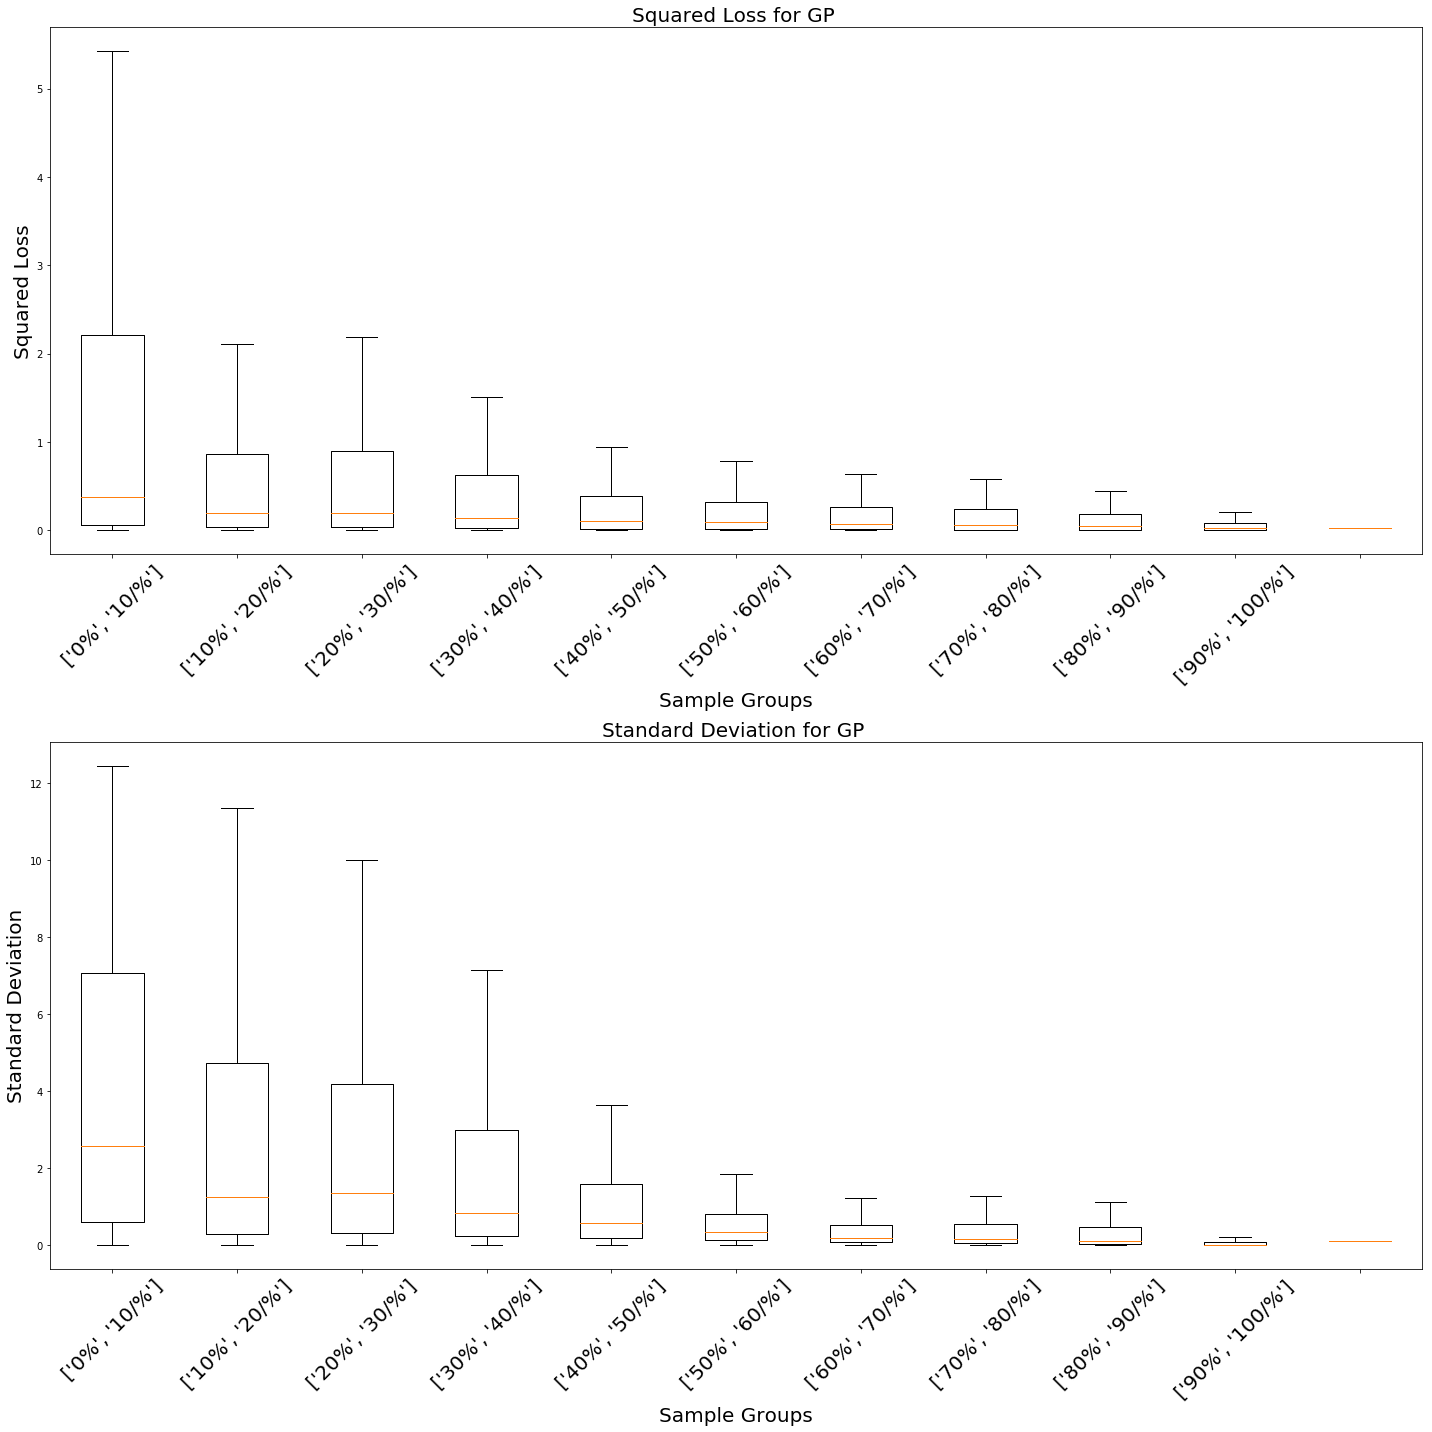
\includegraphics[width=0.5\textwidth]{PLT/sarcos_gpbox.png}
\caption{SARCO: box plot of mean squared loss and standard deviation of GP}
\label{fig:sarcos_gpbox}
\end{figure}


% In this example we consider learning the inverse dynamics of a seven degrees-of- freedom SARCOS robot arm1. The task is to map from a 21-dimensional input space (7 joint positions, 7 joint velocities, 7 joint accelerations) to the corresponding 7 joint torques. Following previous studies on this benchmark (see references in [14]) we only consider the mapping to the first of the seven torques, that is, we learn a function f : R21 → R. There are 44,484 training examples and 4,449 test examples. All 21 inputs xi have been standardized to have zero mean and standard deviation 1. The output y has zero mean. Results are given as standardized mean squared error (SMSE), which is the mean squared error on the test set divided by the variance of the target values in the test set. The normalization by the variance makes the error measure independent on the overall scale of the target.
% While in a real safety-related application the worst-case error should be consid- ered additionally to the mean error, here we solely use the SMSE to facilitate the comparison with previous studies.
% All methods described in the following were applied to this benchmark. The re- sulting SMSE accuracy is summarized in Table 1.

